%%%%%%%%%%%%%%%%%%%%%%%%%%%%%%%%%%%%%%%%%
% baposter Landscape Poster
% LaTeX Template
% Version 1.0 (11/06/13)
%
% baposter Class Created by:
% Brian Amberg (baposter@brian-amberg.de)
%
% This template has been downloaded from:
% http://www.LaTeXTemplates.com and modified by Antonius Torode
%
% License:
% CC BY-NC-SA 3.0 (http://creativecommons.org/licenses/by-nc-sa/3.0/)
%
%%%%%%%%%%%%%%%%%%%%%%%%%%%%%%%%%%%%%%%%%

%----------------------------------------------------------------------------------------
%	PACKAGES AND OTHER DOCUMENT CONFIGURATIONS
%----------------------------------------------------------------------------------------

\documentclass[landscape,a0paper,fontscale=0.285]{baposter} % Adjust the font scale/size here

\usepackage{graphicx} % Required for including images
\graphicspath{{figures/}} % Directory in which figures are stored

\usepackage{amsmath} % For typesetting math
\usepackage{amssymb} % Adds new symbols to be used in math mode

\usepackage{booktabs} % Top and bottom rules for tables
\usepackage{enumitem} % Used to reduce itemize/enumerate spacing
\usepackage{palatino} % Use the Palatino font
\usepackage[font=small,labelfont=bf]{caption} % Required for specifying captions to tables and figures

\usepackage{multicol} % Required for multiple columns
\setlength{\columnsep}{1.5em} % Slightly increase the space between columns
\setlength{\columnseprule}{0mm} % No horizontal rule between columns

\usepackage{tikz} % Required for flow chart
\usetikzlibrary{shapes,arrows} % Tikz libraries required for the flow chart in the template

\newcommand{\compresslist}{ % Define a command to reduce spacing within itemize/enumerate environments, this is used right after \begin{itemize} or \begin{enumerate}
\setlength{\itemsep}{1pt}
\setlength{\parskip}{0pt}
\setlength{\parsep}{0pt}
}

\definecolor{lightblue}{rgb}{0.145,0.6666,1} % Defines the color used for content box headers


\begin{document}
	
\background{%
	\begin{tikzpicture}
	[remember picture,overlay]\node[opacity=1] at (current page.center) {
\includegraphics[width=\paperwidth,height=\paperheight]{BG3.jpg}};
	\end{tikzpicture}%
}

\begin{poster}
{
headerborder=closed, % Adds a border around the header of content boxes
colspacing=1em, % Column spacing
background=user,
%bgColorOne=white, % Background color for the gradient on the left side of the poster
%bgColorTwo=white, % Background color for the gradient on the right side of the poster
borderColor=lightblue, % Border color
headerColorOne=black, % Background color for the header in the content boxes (left side)
headerColorTwo=lightblue, % Background color for the header in the content boxes (right side)
headerFontColor=white, % Text color for the header text in the content boxes
boxColorOne=white, % Background color of the content boxes
textborder=roundedleft, % Format of the border around content boxes, can be: none, bars, coils, triangles, rectangle, rounded, roundedsmall, roundedright or faded
eyecatcher=true, % Set to false for ignoring the left logo in the title and move the title left
headerheight=0.1\textheight, % Height of the header
headershape=roundedright, % Specify the rounded corner in the content box headers, can be: rectangle, small-rounded, roundedright, roundedleft or rounded
headerfont=\Large\bf\textsc, % Large, bold and sans serif font in the headers of content boxes
%textfont={\setlength{\parindent}{1.5em}}, % Uncomment for paragraph indentation
linewidth=2pt % Width of the border lines around content boxes
}
%----------------------------------------------------------------------------------------
%	TITLE SECTION 
%----------------------------------------------------------------------------------------
%
{
\includegraphics[height=4em]{MSU.jpg}} % First university/lab logo on the left
{\bf\textsc{Zeeman Effect on The Hydrogen Atom}\vspace{0.5em}} % Poster title
{\textsc{Antonius Torode and Eric Aboud \\ Michigan State University - Department of Physics \& Astronomy}} % Author names and institution
{
\includegraphics[height=4em]{MSU.jpg}} % Second university/lab logo on the right

%----------------------------------------------------------------------------------------
%	OBJECTIVES
%----------------------------------------------------------------------------------------

\headerbox{Introduction \& History}{name=objectives,column=0,row=0}{

The Zeeman effect comes about from putting an atom in a magnetic field. The magnetic field causes a magnetic moment to be produced and perturbs the energy levels of the atom causing spectral line shifts to appear when modeled or measured with spectroscopy.

\vspace{0.3em} % When there are two boxes, some whitespace may need to be added if the one on the right has more content
}

%----------------------------------------------------------------------------------------
%	Discovery & Properties
%----------------------------------------------------------------------------------------

\headerbox{Observations }{name=introduction,column=3,row=0,bottomaligned=objectives}{
The Zeeman Effect is a real phenomenon that can be observed in spectroscopy when magnetic fields effect the radiation (see figure 3). This can be used to determine where magnetic fields are present and their strength depending on the separation of observed spectral energy levels.
}

%----------------------------------------------------------------------------------------
%	Perturbation Theory \& The Zeeman Effect
%----------------------------------------------------------------------------------------

\headerbox{Perturbation Theory \& The Zeeman Effect}{name=results,column=1,span=2,row=0}{

\begin{multicols}{2}
	The unperturbed Hamiltonian of hydrogen is given by 
	\begin{align}
	H^{(0)} = \underbrace{\frac{\vec{p}^2}{2m}}_{\textrm{Kinetic term}}-\underbrace{\frac{\hbar c \alpha}{r}}_{\textrm{Potential term}}.
	\end{align}
	The total Zeeman Effect to the Hamiltonian are given by determining the effect of a constant magnetic field $\vec{B}$,
	\begin{align}
	H_{mag}^{(1)}= \frac{e}{2m}(\vec{L}+2\vec{S})\cdot \vec{B} = \frac{\mu_B}{\hbar}(\vec{L}+2\vec{S})\cdot \vec{B},
	\end{align} 
	where $\mu_B=\frac{e\hbar}{2m}$ is the Bohr magneton. From perturbation theory we can solve for the first order energy corrections that come from $H_{mag}^{(1)}$ by using 
	\begin{align}
	E_{n}^{(1)} &= \langle n j m_j \ell s| H_{mag}^{(1)}|n j m_j \ell s \rangle.
	\end{align}
	This gives a general result 
	\begin{align}
	E_{n}^{(1)}  = \mu_BBm_jg_L, \label{E_{n}^{(1)}}
	\end{align}
	where $g_L$ is the Land\'{e} g factor. This result in (\ref{E_{n}^{(1)}}) can be used for an explicit state of the hydrogen atom. For example, consider the $2P_{3/2}$ state. This has $n=2$, $\ell =1$, $s=\frac{1}{2}$, and $j=\frac{3}{2}$. The $m_j$ values are shown by the set $m_j = \{-\frac{3}{2},-\frac{1}{2}, \frac{1}{2}, \frac{3}{2} \}$, which tells us there will be 4 different energy splits for this state. Using these values gives us a $g_L=\frac{4}{3}$ and so our energy splits are
	\begin{align}
	E_{2P_{3/2}}^{(1)} = \begin{cases}
	2\mu_BB & \textrm{for }m_j = \frac{3}{2}\\ 
	\frac{2\mu_BB}{3} & \textrm{for }m_j = \frac{1}{2} \\
	-\frac{2\mu_BB}{3}& \textrm{for }m_j = -\frac{1}{2} \\
	-2\mu_BB & \textrm{for }m_j = -\frac{3}{2}
	\end{cases}  \label{l=1 energies}
	\end{align}
\end{multicols}
\vspace{0.01cm}
}

%----------------------------------------------------------------------------------------
%	REFERENCES LEFT
%----------------------------------------------------------------------------------------

\headerbox{References}{name=references,column=0,above=bottom}{


\scriptsize{ % Reduce the font size in this block
\begin{enumerate}
\itemsep0em 
\item Griffiths, David J. Introduction to Quantum Mechanics. 2nd ed. Harlow: Pearson, 2014. Print.
\item Image from https://en.wikipedia.org/wiki/Zeeman\_effect
\end{enumerate}
\vspace{0.5cm}
}}

%----------------------------------------------------------------------------------------
%	Addendum and Final Remarks
%----------------------------------------------------------------------------------------

\headerbox{Addendum and Final Remarks }{name=futureresearch,column=1,span=2,aligned=references,above=bottom}{ % This block is as tall as the references block
As shown above, the induced electric field of a linearly changing magnetic field in time does not induce the Stark Effect. For any constant magnetic field, we are able to generate a plot of the correction splittings as shown in figure 4 and 5. It is important to note that with a time dependent magnetic field, we would need to use time-dependent perturbation theory to solve for the energy corrections.
}


%----------------------------------------------------------------------------------------
%	Changing Magnetic Fields \& Induced Electric Fields
%----------------------------------------------------------------------------------------

\headerbox{Changing Magnetic Fields \& Induced Electric Fields}{name=conclusion,column=1,span=2,row=0,below=results,above=references}{

\begin{multicols}{3}
Consider $\vec{B} = Bt \hat{z}$. By Maxwell's Equations we have $\frac{\partial \vec{E}}{\partial t} = 0$, which implies the electric field is a constant throughout time. Similarly, the electric field must satisfy $\nabla \times \vec{E} = -B \hat{z}$. If we take the curl of both sides of this we get
\begin{align*}
\nabla \times(\nabla \times \vec{E}) &= \nabla (\nabla \cdot \vec{E})- \nabla^2 \vec{E} \\ &= -\nabla \times B \hat{z} =0.
\end{align*}
Using the assumption of a vacuum, this becomes 
\begin{align*}
\nabla^2 \vec{E} =  0 \label{del^2 E=0}
\end{align*}
From this and our magnetic field, we require that there be an electric field $\vec{E}_1=By \hat{x}$ in order for Maxwell's equations to be satisfied. By analogy we can also find another solution to $\vec{E}$ as $\vec{E}_2 = -Bx\hat{y}$. And so by superposition we can also have a solution
\begin{align}
\vec{E}_{1+2} = B(y \hat{x}-x\hat{y}).
\end{align}
This shows that with a changing magnetic field, we would see an electric field appear which could itself cause another corrections to the perturbed energies. This is known as the Stark Effect and in our case would introduce the correction
\begin{align}
H_{elec}^{(1)}=-e\vec{r}\cdot\vec{E}=0.
\end{align} 

\begin{center}
	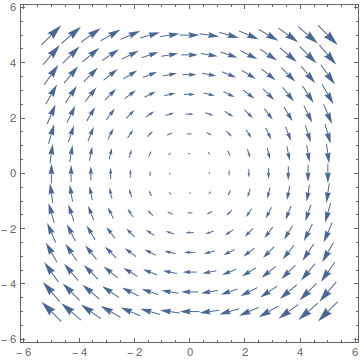
\includegraphics[width=0.22\textwidth]{E1plus2.png}
	
	{\footnotesize \textbf{Figure 2.} A plot of $\vec{E}_{1+2}$ using B=1 in the x-y plane.}
\end{center}
\end{multicols}
}

%----------------------------------------------------------------------------------------
%	Computational Models
%----------------------------------------------------------------------------------------

\headerbox{Computational Models}{name=method,column=3,below=objectives,bottomaligned=references}{ % This block's bottom aligns with the bottom of the conclusion block
\small{
	
\begin{center}
	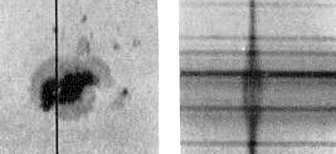
\includegraphics[width=0.75\linewidth]{figures/observed}
	
	{\footnotesize \textbf{Figure 3.} Observations of the Zeeman Effect from spectroscopy of a sunspot [2].}
	
	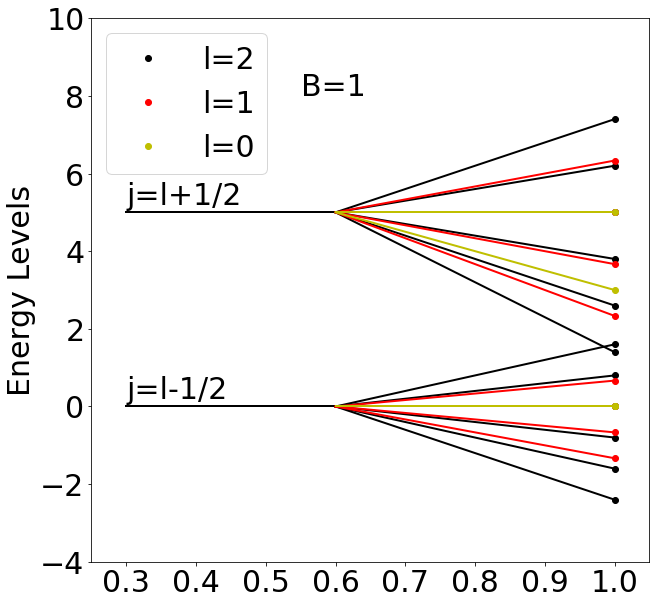
\includegraphics[width=0.75\linewidth]{figures/Bis1}
	
	{\footnotesize \textbf{Figure 4.} Relative hydrogen Energy corrections.}
	
	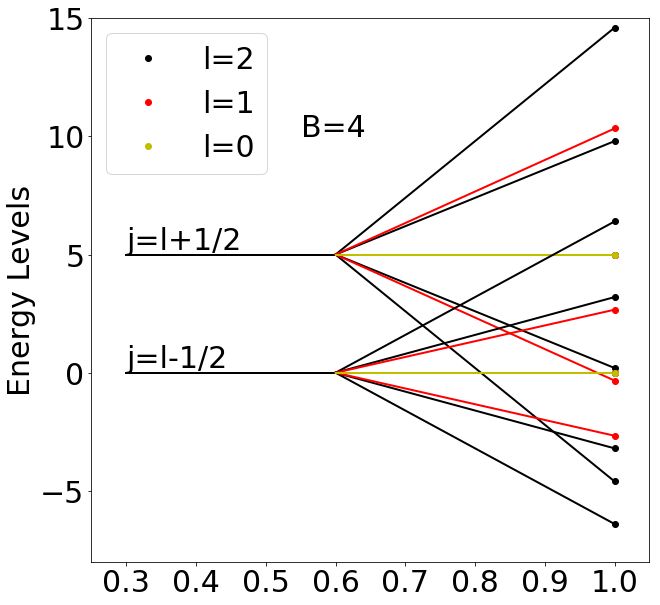
\includegraphics[width=0.75\linewidth]{figures/Bis4}
	
	{\footnotesize \textbf{Figure 5.} Relative hydrogen Energy corrections with an increased magnetic field.}
\end{center}
	
	

}}

%----------------------------------------------------------------------------------------
%	Land\'{e}  g Factor
%----------------------------------------------------------------------------------------

\headerbox{Land\'{e}  g Factor}{name=results2,column=0,below=objectives,bottomaligned=conclusion}{ % This block's bottom aligns with the bottom of the conclusion block
\small{
Consider the Land\'{e} g factor for the hydrogen atom Zeeman Effect with a spin value of $s=\frac{1}{2}$,
\begin{align}
g_L = \frac{12j(j+1)-4\ell(\ell+1)+3}{8j(j+1)}.
\end{align}
Now, $m_j = \{j+k|-j \leq m_j \leq j \textrm{ and } k \in \mathbb{Z}\}$ which can be expressed in terms of $\ell$ as
\begin{align*}
m_j = \{\ell \pm \frac{1}{2}+k|-\ell \leq m_j\pm \frac{1}{2} \leq \ell \pm 1 \textrm{ and } k \in \mathbb{Z}\}.
\end{align*}
Using these two forms of $m_j$ and $g_L$, we can write out energy corrections in terms of a single variable for both $j=\ell+\frac{1}{2}$ and $j=\ell-\frac{1}{2}$ respectively as,
\begin{align*}
E_{n}^{(1)} = \mu_BB\begin{cases}
	\frac{2+2l}{1+2\ell}(\ell + \frac{1}{2}-k) & \textrm{for } 0 \leq k \leq 2\ell+1\\
	\frac{2l}{1+2\ell}(\ell - \frac{1}{2}-k) & \textrm{for } 0 \leq k \leq 2\ell-1
	\end{cases}.
\end{align*}
Now we have a general formula for the corrected energy levels that we can plot for any $\ell$ value for spin $s=\frac{1}{2}$ hydrogen (demonstrated in figure 1).
\begin{center}
	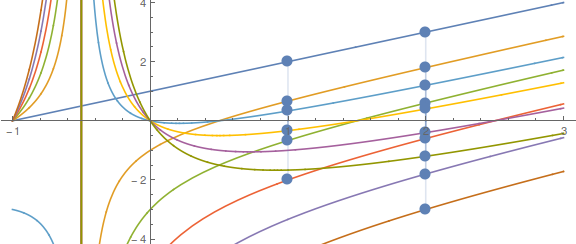
\includegraphics[width=0.8\textwidth]{figures/Energylevelstrimmed.png}
	
	{\footnotesize \textbf{Figure 1.} Relative hydrogen Energy corrections for $\ell=1$ and $\ell=2$ with units of $\mu_B=B=1$.}
\end{center}
}}

%----------------------------------------------------------------------------------------

\end{poster}

\end{document}